% !TeX root = ..\G16.tex
\section{Design}
\subsection{MVC}\label{MVC}
Vi har som løsning til opgaven valgt at lave 3 klasser. Disse klasser er skabt efter 'Model-View-Controller' - mønsteret. Derudover har vi også en .fxml fil, der indeholder al information om vores stage og scene. Denne fil redigeres igennem scene-builder. Et alternativ til scene-builder kunne være, at skrive hele koden for det visuelle i javafx. Dette vælger vi dog ikke at gøre, da det, i vores optik, vil være mere praktisk at designe det grafiske i scene-builder, da man kan placere diverse objekter/nodes som 'Buttons', 'Panes' osv. på 'scene' og redigere dem, uden at skulle have en eksakt viden om de specifikke koordinater, hvorpå vi stiller dem, og uden at skulle skrive deres længder, bredder osv. ned. Vores klasser er de tre følgende:
\subsubsection{Main}
En main-klasse, der fungerer som view; altså alt det, som spilleren kan se. Den sætter altså programmet igang, viser stage, scene, nodes osv. En board-klasse, der fungerer som model; den står for alt al logik, der bruges til at implementerer de forskellige regler og funktioner ved spillet, som f.eks. at vende brikker, der er indeklemte, eller at afgøre, om hvorvidt man kan stille en brik på et bestemt felt. 
\subsubsection{Controller}
En controller-klasse, der fungerer controller; denne klasse binder board og .fxml-filen sammen. Dette gør den ved at lave en masse metoder, der responderer på et klik med musen eller et klik på en "Button" på "scene", således at der sker nogle ændringer visuelt, og disse ændringer har forklaring med rod i logikken (board-klassen).
\subsubsection{Board}
\begin{figure}[H]
    \centering
    \caption{Model Viewer Controller konceptet (af Rafael D. Hernandez) \href{https://www.freecodecamp.org/news/the-model-view-controller-pattern-mvc-architecture-and-frameworks-explained/}{freecodecamp.org})}\label{fig:my_label}
    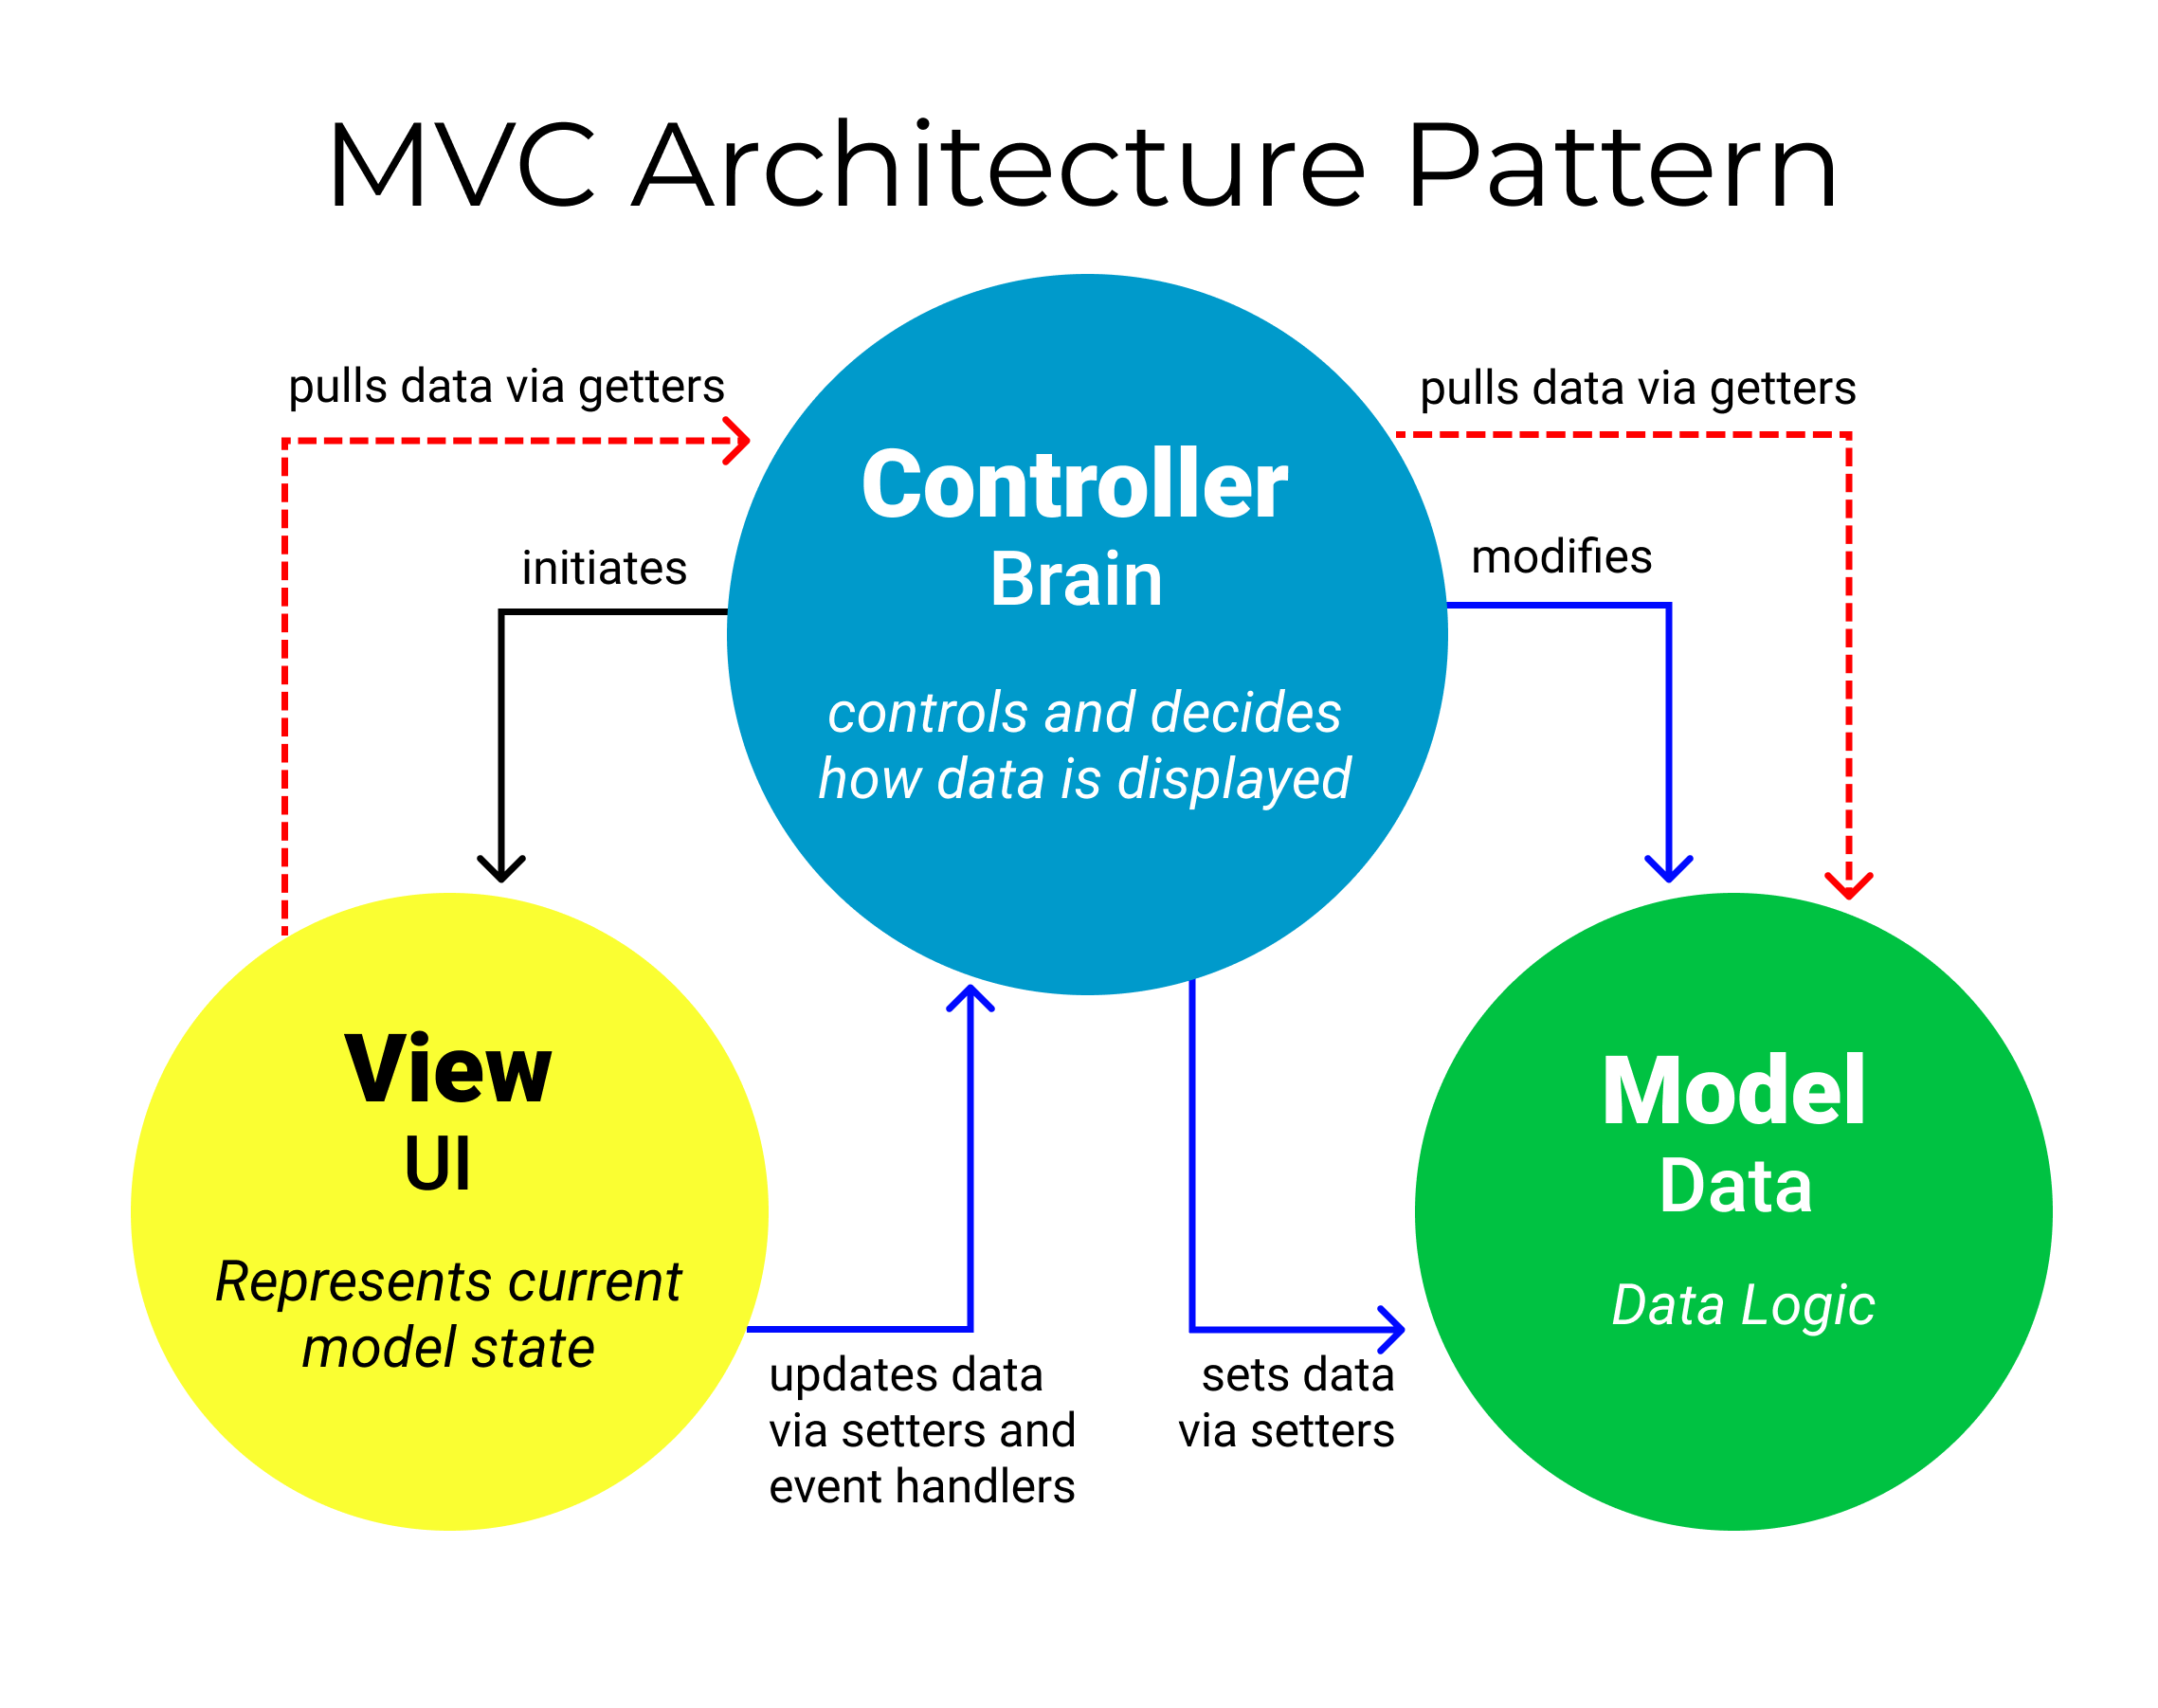
\includegraphics[width=.5\textwidth]{Graphics/MVC3.png}
\end{figure}

Som en tilføjelse, der ikke vil indgå i den endelige aflevering, og som ikke indgår i eksekveringen af de tre klasser for oven, laver vi også en board-driver klasse, der vil være i stand til at kunne teste "board" klassens funktionsdygtighed. Dette gør vi, eftersom der ikke vil være mulighed for at teste logikken rent visuelt, før controller/scene-builder delen er færdig. Dette skyldes, at controller-klassen modtager og arbejder med data fra board, og hvis controllerklassen så ikke er færdig, er den ikke i stand til at gøre dette på en ordentlig måde. 

